\documentclass[tikz,border=6pt]{standalone}
\usepackage{amsmath,amssymb,mathtools,physics,bm,nicefrac,wasysym}
\usepackage{xcolor}

\definecolor{colone}{RGB}{180,60,60}
\definecolor{coltwo}{RGB}{60,110,180}
\definecolor{colthree}{RGB}{60,140,80}

\definecolor{accent}{HTML}{A13D2C}
\definecolor{accent2}{HTML}{2B5F6B}
\definecolor{muted}{HTML}{5A564F}
\definecolor{panel}{HTML}{F8F6F0}
\definecolor{linecol}{HTML}{D8D2C4}
\definecolor{ink}{HTML}{1E1C1A}
\definecolor{astroblue}{HTML}{1B4F72}
\definecolor{astrodark}{HTML}{17202A}
\definecolor{sunyellow}{HTML}{E8A33D}

\usetikzlibrary{calc,arrows.meta,positioning,decorations.pathreplacing,decorations.markings,angles,quotes,shapes.geometric}
\usepackage{tikz-3dplot}

\newcommand{\vecr}{\vec r}
\newcommand{\vecL}{\vec L}
\newcommand{\vecA}{\vec A}
\newcommand{\vecf}{\vec f}
\newcommand{\vecF}{\vec F}
\newcommand{\vecp}{\vec p}
\newcommand{\avg}[1]{\left\langle #1\right\rangle}
\newcommand{\vecx}{\vec x}
\newcommand{\hatn}{\hat n}
\newcommand{\rhat}{\hat r}
\newcommand{\phihat}{\hat\phi}
\newcommand{\thetahat}{\hat\theta}
\newcommand{\note}[1]{\textcolor{blue!60!black}{\textit{[#1]}}}

\newcommand{\LST}{\mathrm{LST}}
\newcommand{\GST}{\mathrm{GST}}
\newcommand{\GMST}{\mathrm{GMST}}
\newcommand{\GAST}{\mathrm{GAST}}
\newcommand{\LMST}{\mathrm{LMST}}
\newcommand{\LAST}{\mathrm{LAST}}
\newcommand{\UT}{\mathrm{UT}}
\newcommand{\UTC}{\mathrm{UTC}}
\newcommand{\TAI}{\mathrm{TAI}}
\newcommand{\TT}{\mathrm{TT}}
\newcommand{\TDB}{\mathrm{TDB}}
\newcommand{\JD}{\mathrm{JD}}
\newcommand{\MJD}{\mathrm{MJD}}
\newcommand{\EoT}{\mathrm{EoT}}
\newcommand{\SNR}{\mathrm{SNR}}
\newcommand{\RON}{\mathrm{RON}}



\begin{document}
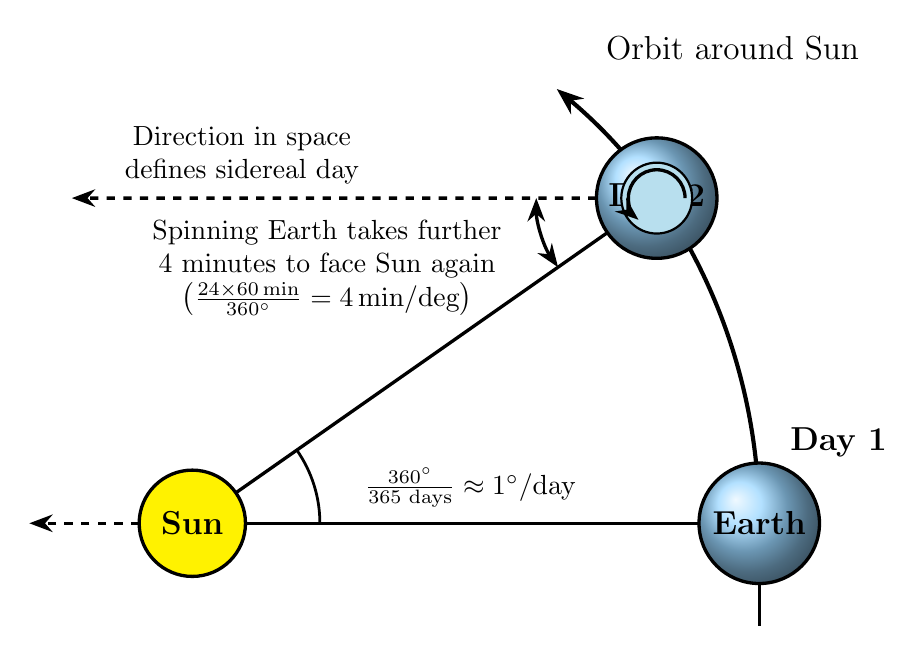
\begin{tikzpicture}[>=Stealth, font=\sffamily, scale=0.9]
    		% Sun at (-1.5, 0), Radius R = 8.0
    		\coordinate (Sun) at (-1.5, 0);
    		\coordinate (Earth1) at (6.5, 0);                 % theta = 0 deg
    		\coordinate (Earth2) at (5.0532, 4.5886);         % theta = 35 deg, R = 8.0
    		
    		% Lines from Sun to Earths
    		\draw[line width=1.2pt] (Sun) -- (Earth1);
    		\draw[line width=1.2pt] (Sun) -- (Earth2);
    		
    		% Parametrized Orbit Arc
    		\draw[line width=1.5pt, ->] (Sun) ++(-5:8.0) arc[start angle=-5, end angle=50, radius=8.0];
    		\node[font=\large, anchor=south west] at (4.2, 6.4) {Orbit around Sun};
    		
    		% Sun
    		\draw[fill=yellow, line width=1.2pt] (Sun) circle (0.75);
    		\node[font=\bfseries\large] at (Sun) {Sun};
    		\draw[dashed, ->, line width=1.2pt] (-2.25, 0) -- (-3.8, 0);
    		
    		% Earth Day 1
    		\shade[ball color=cyan!60!blue!40] (Earth1) circle (0.85);
    		\draw[line width=1.2pt] (Earth1) circle (0.85);
    		\node[font=\bfseries\large] at (Earth1) {Earth};
    		\node[font=\bfseries\large, anchor=south west] at (6.8, 0.8) {Day 1};
    		\draw[line width=1.2pt] (6.5, -0.85) -- (6.5, -1.45);
    		
    		% Earth Day 2
    		\shade[ball color=cyan!60!blue!40] (Earth2) circle (0.85);
    		\draw[line width=1.2pt] (Earth2) circle (0.85);
    		\node[font=\bfseries\large] at (Earth2) {Day 2};
    		
    		% Inner core + spin arrow on Earth 2
    		\draw[fill=cyan!80!black!30, line width=0.8pt] (Earth2) circle (0.5);
    		\draw[->, line width=1.2pt] (Earth2) ++(0:0.4) arc[start angle=0, end angle=230, radius=0.4];
    		
    		% Dashed Sidereal Direction Line from Earth 2
    		\draw[dashed, ->, line width=1.2pt] (Earth2) ++(-0.85, 0) -- (-3.2, 4.5886);
    		\node[align=center, font=\normalsize, anchor=south] at (-0.8, 4.65) {Direction in space\\defines sidereal day};
    		
    		% Angles & Annotations
    		\draw[line width=1pt] (Sun) ++(1.8, 0) arc[start angle=0, end angle=35, radius=1.8];
    		\node[font=\normalsize, anchor=west] at (0.8, 0.5) {$\frac{360^{\circ}}{365\text{ days}}\approx 1^\circ/\text{day}$};
    		
    		% Angle at Earth 2
    		\draw[<->, line width=1.2pt] (Earth2) ++(180:1.7) arc[start angle=180, end angle=215, radius=1.7];
    		\node[align=center, font=\normalsize, anchor=east] at (3.0, 3.6) {Spinning Earth takes further\\$4$ minutes to face Sun again\\
    			$\left(\frac{24\times 60\,\text{min}}{360^{\circ}}=4\,\text{min/deg}\right)$};
    	\end{tikzpicture}
\end{document}
